%include part: see main.beamer.tex and main.article.tex
%include common packages and settings
\usepackage{etex} %эта магическая херь избавляет от переполнения регистров TeX а!!!

\mode<article>{\usepackage{fullpage}}
\mode<presentation>{
    \usetheme{Madrid} %%Boadilla,Madrid,AnnArbor,CambridgeUS,Malmoe,Singapore,Berlin
    \useoutertheme{shadow}
} 

\usepackage[utf8]{inputenc}
\usepackage[russian]{babel}
\usepackage{indentfirst}
\usepackage{graphicx}

\usepackage{amsmath}
\usepackage{amsfonts}
\usepackage{amsthm}
\usepackage{algorithm}
\usepackage{algorithmic}

\usepackage[all]{xy}

\date{Лекция по дисциплине <<информатика>>\\(\today)}
\author[М.~М.~Шихов]{Михаил Шихов \\ \texttt{\underline{m.m.shihov@gmail.com}}}

%для рисования графов пакетом xy-pic
\entrymodifiers={++[o][F-]}

%для псевдокода алгоритмов (algorithm,algorithmic)
\renewcommand{\algorithmicrequire}{\textbf{Вход:}}
\renewcommand{\algorithmicensure}{\textbf{Выход:}}
\renewcommand{\algorithmiccomment}[1]{// #1}
\floatname{algorithm}{Псевдокод}

%%определённые мной команды логической разметки
\newcommand{\DC}[1]{\text{ДК}(#1)}
\newcommand{\MDC}[1]{\text{MДК}(#1)}
\newcommand{\OC}[1]{\text{ОК}(#1)}
\newcommand{\MOC}[1]{\text{МОК}(#1)}
\newcommand{\PC}[1]{\text{ПК}(#1)}

\newcommand{\Machine}[1]{\texttt{#1}}

\newcommand{\UnsignedAny}[2]{\text{\upshape
    \begin{tabular}{lr}
        \tiny{#1} & \tiny{0}\\ 
        \hline
        \multicolumn{2}{|c|}{\Machine{#2}} \\ 
        \hline
    \end{tabular}
}}

\newcommand{\UnsignedByte}[1]{\UnsignedAny{7}{#1}}

\newcommand{\UnsignedTwoBytes}[1]{\UnsignedAny{15}{#1}}

\newcommand{\SignedAny}[4]{\text{\upshape
    \begin{tabular}{clr}
        \tiny{#1}  &\tiny{#2} & \tiny{0}\\ 
        \hline
        \multicolumn{1}{|c|}{\Machine{#3}} & \multicolumn{2}{|c|}{\Machine{#4}} \\ 
        \hline
    \end{tabular}
}}

\newcommand{\SignedNibble}[2]{\SignedAny{3}{2}{#1}{#2}}

\newcommand{\SignedByte}[2]{\SignedAny{7}{6}{#1}{#2}}

\newcommand{\SignedTwoBytes}[2]{\SignedAny{15}{14}{#1}{#2}}

\newcommand{\FloatMyHex}[4]{\text{\upshape
    \begin{tabular}{clrclr}
        \tiny{15}  &\tiny{14} & \tiny{6} & \tiny{5} & \tiny{4} & \tiny{0}\\ 
        \hline
        \multicolumn{1}{|c|}{\texttt{#1}} 
            & \multicolumn{2}{|c|}{\texttt{#2}} 
                & \multicolumn{1}{|c|}{\texttt{#3}} 
                    & \multicolumn{2}{|c|}{\texttt{#4}} \\ 
        \hline
    \end{tabular}
}}

\newcommand{\FloatMyCharHex}[3]{\text{\upshape
    \begin{tabular}{clrlr}
        \tiny{15}  &\tiny{14} & \tiny{6} & \tiny{5} & \tiny{0}\\ 
        \hline
        \multicolumn{1}{|c|}{\texttt{#1}} 
            & \multicolumn{2}{|c|}{\texttt{#2}} 
                & \multicolumn{2}{|c|}{\texttt{#3}} \\ 
        \hline
    \end{tabular}
}}

\newcommand{\FloatMySimpleHex}[2]{\text{\upshape
    \begin{tabular}{lrlr}
        \tiny{15}  & \tiny{6} & \tiny{5} & \tiny{0} \\ 
        \hline
        \multicolumn{2}{|c|}{\texttt{#1}} 
            & \multicolumn{2}{|c|}{\texttt{#2}} \\ 
        \hline
    \end{tabular}
}}

\newcommand{\FloatMyOrderX}[4]{\text{\upshape
    \begin{tabular}{clrclr}
        \tiny{9}  &\tiny{8} & \tiny{4} & \tiny{3} & \tiny{2} & \tiny{0}\\ 
        \hline
        \multicolumn{1}{|c|}{\texttt{#1}} 
            & \multicolumn{2}{|c|}{\texttt{#2}} 
                & \multicolumn{1}{|c|}{\texttt{#3}} 
                    & \multicolumn{2}{|c|}{\texttt{#4}} \\ 
        \hline
    \end{tabular}
}}

\newcommand{\FloatMyDcOrderX}[3]{\text{\upshape
    \begin{tabular}{lrclr}
        \tiny{9} & \tiny{4} & \tiny{3} & \tiny{2} & \tiny{0}\\ 
        \hline
        \multicolumn{2}{|c|}{\texttt{#1}} 
            & \multicolumn{1}{|c|}{\texttt{#2}} 
                & \multicolumn{2}{|c|}{\texttt{#3}} \\ 
        \hline
    \end{tabular}
}}

\newcommand{\FloatMyDcCharX}[2]{\text{\upshape
    \begin{tabular}{lrlr}
        \tiny{9} & \tiny{4} & \tiny{3} & \tiny{0}\\ 
        \hline
        \multicolumn{2}{|c|}{\texttt{#1}} 
            & \multicolumn{2}{|c|}{\texttt{#2}} \\ 
        \hline
    \end{tabular}
}}

\newcommand{\FloatMyCharX}[3]{\text{\upshape
    \begin{tabular}{clrlr}
        \tiny{9}  &\tiny{8} & \tiny{4} & \tiny{3} & \tiny{0}\\ 
        \hline
        \multicolumn{1}{|c|}{\texttt{#1}} 
            & \multicolumn{2}{|c|}{\texttt{#2}} 
                & \multicolumn{2}{|c|}{\texttt{#3}} \\ 
        \hline
    \end{tabular}
}}

\newcommand{\FloatESShort}[3]{\text{\upshape
    \begin{tabular}{clrlr}
        \tiny{31}  &\tiny{30} & \tiny{24} & \tiny{23} & \tiny{0}\\ 
        \hline
        \multicolumn{1}{|c|}{\texttt{#1}} 
            & \multicolumn{2}{|c|}{\texttt{#2}} 
                & \multicolumn{2}{|c|}{\texttt{#3}} 
                    \\ 
        \hline
    \end{tabular}
}}

\newcommand{\FloatPCShort}[3]{\text{\upshape
    \begin{tabular}{clrlr}
        \tiny{31}  &\tiny{30} & \tiny{23} & \tiny{22} & \tiny{0}\\ 
        \hline
        \multicolumn{1}{|c|}{\texttt{#1}} 
            & \multicolumn{2}{|c|}{\texttt{#2}} 
                & \multicolumn{2}{|c|}{\texttt{#3}} 
                    \\ 
        \hline
    \end{tabular}
}}


%--- СПЕЦИФИЧНЫЕ ДЛЯ УМНОЖЕНИЯ КОМАНДЫ ---------------------------------------------------------------------------------------------


\newcommand{\Number}[1]{
    \texttt{#1}
}

\newcommand{\NumberHi}[2]{
    \underline{\underline{\texttt{#1}}}\texttt{#2}
}

\newcommand{\NumberMid}[3]{
    \texttt{#1}\underline{\underline{\texttt{#2}}}\texttt{#3}
}

\newcommand{\NumberLo}[2]{
    \texttt{#1}\underline{\underline{\texttt{#2}}}
}

\newcommand{\Stack}[2]{
    \begin{tabular}[t]{@{}r@{}}
        {#1}\\ \hline
        {#2}\\ 
    \end{tabular}
}

\newcommand{\Operation}[4]{
    \begin{tabular}[t]{@{}r@{}}
        \texttt{#4}
        \begin{tabular}{@{}r@{}}
            \Number{#1}\\
            \Number{#2}\\ \hline
        \end{tabular} \\ 
        \Number{#3}\\
    \end{tabular}
}

\newcommand{\Addition}[3]{\Operation{#1}{#2}{#3}{+}}

\newcommand{\Subtraction}[3]{\Operation{#1}{#2}{#3}{-}}

\newcommand{\Multiplication}[3]{\Operation{#1}{#2}{#3}{$\times$}}

\newcommand{\Register}[2]{\Number{#1:#2}}

\newcommand{\Mantiss}{m}
\newcommand{\Order}{p}
\newcommand{\Char}{c}

\newcommand{\MantissOf}[1]{\Mantiss_{#1}}
\newcommand{\OrderOf}[1]{\Order_{#1}}
\newcommand{\CharOf}[1]{\Char_{#1}}

\newcommand{\FloatExpression}[2]{\MantissOf{#1}\cdot {#2}^{\OrderOf{#1}}}

\newenvironment{Solve}[1]%
    {\begin{proof}[Решение]#1}
    {\end{proof}}
    
    
%определённые мной команды логической разметки
\newcommand{\DC}[1]{\text{ДК}(#1)}
\newcommand{\MDC}[1]{\text{MДК}(#1)}
\newcommand{\OC}[1]{\text{ОК}(#1)}
\newcommand{\MOC}[1]{\text{МОК}(#1)}
\newcommand{\PC}[1]{\text{ПК}(#1)}

\newcommand{\Machine}[1]{\texttt{#1}}

\newcommand{\UnsignedAny}[2]{\text{\upshape
    \begin{tabular}{lr}
        \tiny{#1} & \tiny{0}\\ 
        \hline
        \multicolumn{2}{|c|}{\Machine{#2}} \\ 
        \hline
    \end{tabular}
}}

\newcommand{\UnsignedByte}[1]{\UnsignedAny{7}{#1}}

\newcommand{\UnsignedTwoBytes}[1]{\UnsignedAny{15}{#1}}

\newcommand{\SignedAny}[4]{\text{\upshape
    \begin{tabular}{clr}
        \tiny{#1}  &\tiny{#2} & \tiny{0}\\ 
        \hline
        \multicolumn{1}{|c|}{\Machine{#3}} & \multicolumn{2}{|c|}{\Machine{#4}} \\ 
        \hline
    \end{tabular}
}}

\newcommand{\SignedNibble}[2]{\SignedAny{3}{2}{#1}{#2}}

\newcommand{\SignedByte}[2]{\SignedAny{7}{6}{#1}{#2}}

\newcommand{\SignedTwoBytes}[2]{\SignedAny{15}{14}{#1}{#2}}

\newcommand{\FloatMyHex}[4]{\text{\upshape
    \begin{tabular}{clrclr}
        \tiny{15}  &\tiny{14} & \tiny{6} & \tiny{5} & \tiny{4} & \tiny{0}\\ 
        \hline
        \multicolumn{1}{|c|}{\texttt{#1}} 
            & \multicolumn{2}{|c|}{\texttt{#2}} 
                & \multicolumn{1}{|c|}{\texttt{#3}} 
                    & \multicolumn{2}{|c|}{\texttt{#4}} \\ 
        \hline
    \end{tabular}
}}

\newcommand{\FloatMyCharHex}[3]{\text{\upshape
    \begin{tabular}{clrlr}
        \tiny{15}  &\tiny{14} & \tiny{6} & \tiny{5} & \tiny{0}\\ 
        \hline
        \multicolumn{1}{|c|}{\texttt{#1}} 
            & \multicolumn{2}{|c|}{\texttt{#2}} 
                & \multicolumn{2}{|c|}{\texttt{#3}} \\ 
        \hline
    \end{tabular}
}}

\newcommand{\FloatMySimpleHex}[2]{\text{\upshape
    \begin{tabular}{lrlr}
        \tiny{15}  & \tiny{6} & \tiny{5} & \tiny{0} \\ 
        \hline
        \multicolumn{2}{|c|}{\texttt{#1}} 
            & \multicolumn{2}{|c|}{\texttt{#2}} \\ 
        \hline
    \end{tabular}
}}

\newcommand{\FloatMyOrderX}[4]{\text{\upshape
    \begin{tabular}{clrclr}
        \tiny{9}  &\tiny{8} & \tiny{4} & \tiny{3} & \tiny{2} & \tiny{0}\\ 
        \hline
        \multicolumn{1}{|c|}{\texttt{#1}} 
            & \multicolumn{2}{|c|}{\texttt{#2}} 
                & \multicolumn{1}{|c|}{\texttt{#3}} 
                    & \multicolumn{2}{|c|}{\texttt{#4}} \\ 
        \hline
    \end{tabular}
}}

\newcommand{\FloatMyDcOrderX}[3]{\text{\upshape
    \begin{tabular}{lrclr}
        \tiny{9} & \tiny{4} & \tiny{3} & \tiny{2} & \tiny{0}\\ 
        \hline
        \multicolumn{2}{|c|}{\texttt{#1}} 
            & \multicolumn{1}{|c|}{\texttt{#2}} 
                & \multicolumn{2}{|c|}{\texttt{#3}} \\ 
        \hline
    \end{tabular}
}}

\newcommand{\FloatMyDcCharX}[2]{\text{\upshape
    \begin{tabular}{lrlr}
        \tiny{9} & \tiny{4} & \tiny{3} & \tiny{0}\\ 
        \hline
        \multicolumn{2}{|c|}{\texttt{#1}} 
            & \multicolumn{2}{|c|}{\texttt{#2}} \\ 
        \hline
    \end{tabular}
}}

\newcommand{\FloatMyCharX}[3]{\text{\upshape
    \begin{tabular}{clrlr}
        \tiny{9}  &\tiny{8} & \tiny{4} & \tiny{3} & \tiny{0}\\ 
        \hline
        \multicolumn{1}{|c|}{\texttt{#1}} 
            & \multicolumn{2}{|c|}{\texttt{#2}} 
                & \multicolumn{2}{|c|}{\texttt{#3}} \\ 
        \hline
    \end{tabular}
}}

\newcommand{\FloatESShort}[3]{\text{\upshape
    \begin{tabular}{clrlr}
        \tiny{31}  &\tiny{30} & \tiny{24} & \tiny{23} & \tiny{0}\\ 
        \hline
        \multicolumn{1}{|c|}{\texttt{#1}} 
            & \multicolumn{2}{|c|}{\texttt{#2}} 
                & \multicolumn{2}{|c|}{\texttt{#3}} 
                    \\ 
        \hline
    \end{tabular}
}}

\newcommand{\FloatPCShort}[3]{\text{\upshape
    \begin{tabular}{clrlr}
        \tiny{31}  &\tiny{30} & \tiny{23} & \tiny{22} & \tiny{0}\\ 
        \hline
        \multicolumn{1}{|c|}{\texttt{#1}} 
            & \multicolumn{2}{|c|}{\texttt{#2}} 
                & \multicolumn{2}{|c|}{\texttt{#3}} 
                    \\ 
        \hline
    \end{tabular}
}}


%--- СПЕЦИФИЧНЫЕ ДЛЯ УМНОЖЕНИЯ КОМАНДЫ ---------------------------------------------------------------------------------------------


\newcommand{\Number}[1]{
    \texttt{#1}
}

\newcommand{\NumberHi}[2]{
    \underline{\underline{\texttt{#1}}}\texttt{#2}
}

\newcommand{\NumberMid}[3]{
    \texttt{#1}\underline{\underline{\texttt{#2}}}\texttt{#3}
}

\newcommand{\NumberLo}[2]{
    \texttt{#1}\underline{\underline{\texttt{#2}}}
}

\newcommand{\Stack}[2]{
    \begin{tabular}[t]{@{}r@{}}
        {#1}\\ \hline
        {#2}\\ 
    \end{tabular}
}

\newcommand{\Operation}[4]{
    \begin{tabular}[t]{@{}r@{}}
        \texttt{#4}
        \begin{tabular}{@{}r@{}}
            \Number{#1}\\
            \Number{#2}\\ \hline
        \end{tabular} \\ 
        \Number{#3}\\
    \end{tabular}
}

\newcommand{\Addition}[3]{\Operation{#1}{#2}{#3}{+}}

\newcommand{\Subtraction}[3]{\Operation{#1}{#2}{#3}{-}}

\newcommand{\Multiplication}[3]{\Operation{#1}{#2}{#3}{$\times$}}

\newcommand{\Register}[2]{\Number{#1:#2}}

\newcommand{\Mantiss}{m}
\newcommand{\Order}{p}
\newcommand{\Char}{c}

\newcommand{\MantissOf}[1]{\Mantiss_{#1}}
\newcommand{\OrderOf}[1]{\Order_{#1}}
\newcommand{\CharOf}[1]{\Char_{#1}}

\newcommand{\FloatExpression}[2]{\MantissOf{#1}\cdot {#2}^{\OrderOf{#1}}}

\newenvironment{Solve}[1]%
    {\begin{proof}[Решение]#1}
    {\end{proof}}
    
    

\date{Научно-практическая конференция\\"Семья и школа №27", г.~Киров, \\2018}
\author[А.~Усольцева]{Анастасия Усольцева}

\title[Привниматическое оружие]{Опыт создания и использования привниматического оружия}

\newcommand{\myDevice}{ТРЕНЬК-2}

\begin{document}

%титул и содержание статьи
\mode<article>{\maketitle}

%титул и содержание презентации
\frame<presentation>{\titlepage}


\begin{frame}
    \frametitle{Участники проекта}
    
    \begin{columns}
        \column{.20\textwidth}
        \only<1>{
            \begin{center}
                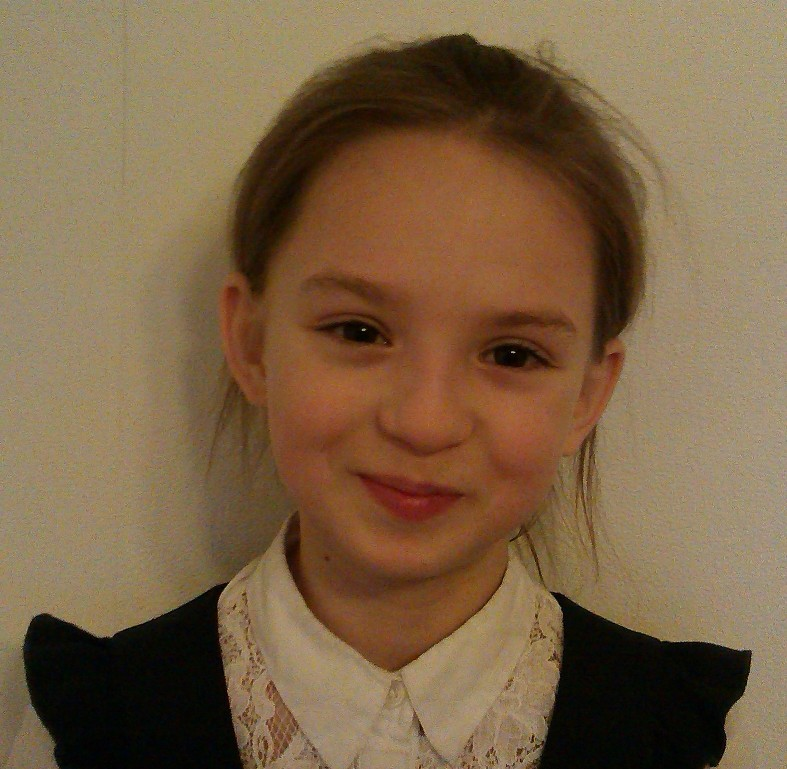
\includegraphics[width=.8\textwidth]{fig/nastyaOfficial}
            \end{center}
        }
        \only<2>{
            \begin{center}
                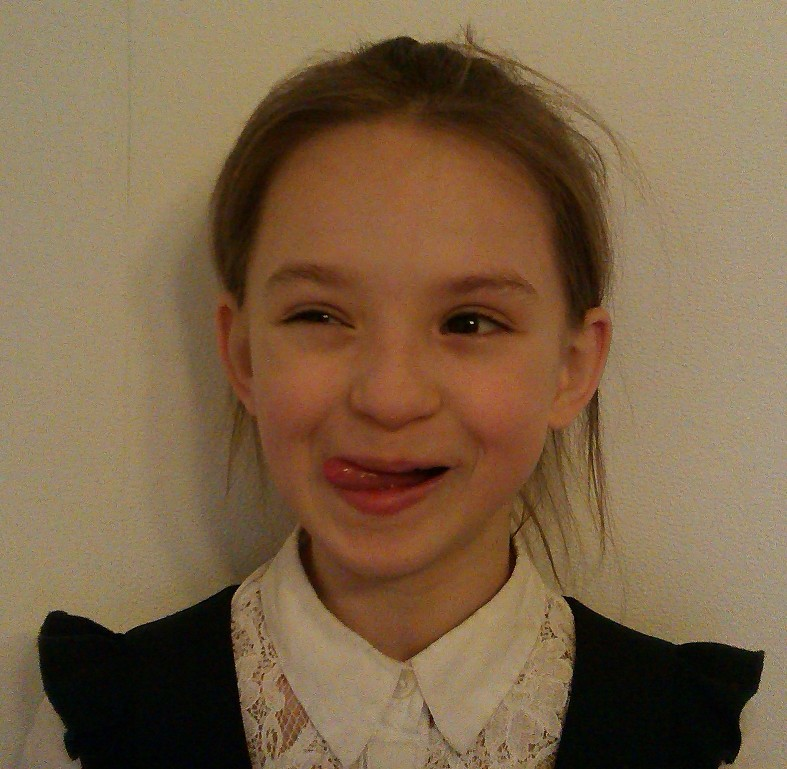
\includegraphics[width=.8\textwidth]{fig/nastyaFox}
            \end{center}
        }
        
        \column{.75\textwidth}
            \alert{Автор и докладчик}: Усольцева Настя, дипломированный хулиган, кандидат привнематических наук, почётный член академии нытиков.
    \end{columns}    
    
    \par\bigskip
    
    \alert{Техническая и моральная поддержка}:
    \begin{itemize}
        \item папа Миша;
        \item мама Оля;
        \item сестра Полина;
        \item кошки (2 шт.);
        \item \alert{КОТ};
        \item собака.
    \end{itemize}
    
\end{frame}

\begin{frame}
    \frametitle{Аннотация}
    
    В работе дается определение и рассматриваются виды \alert{привниматического оружия} (далее будем говорить просто: оружие). 
    
    \par\bigskip
    
    Приводятся \alert{особенности и правила} использования такого оружия. 
    
    \par\bigskip

    Анализируются \alert{существующие модели} оружия. 

    \par\bigskip
    
    Приводится пример разработки и использования модели вниматомета \alert{\myDevice} и дается прогноз направлений развития привниматического оружия.
\end{frame}

Работа не может считаться научной, если в ней нет непонятных слов. Задача настоящего ученого --- использовать только непонятные слова, потому что тогда он кажется умнеее. Придумать новое непонятное слово --- признак настоящего мастера.
    
\begin{frame}
    \frametitle{Введение и обоснование актуальности}
    
    \begin{block}{Определение}
        \par\bigskip
        \alert{$\overbrace{\text{ПРИ}}\overbrace{\text{ВНИ}}\overbrace{\text{МАТИЧЕСКОЕ}}$} оружие --- это оружие, 
        \begin{itemize}
            \item \alert{ПРИ}влекающее 
            \item \alert{ВНИ}мание 
            \item авто\alert{МАТИЧЕСКИ}.
        \end{itemize}
    \end{block}
    
    
    \alert{Внимание} --- это духовный ресурс, которого на всех не хватает. 

    \par\bigskip

    Внимательных людей мало и за внимание людей невнимательных, люди непримечательные издавна воюют между собой. 

    \par\bigskip

    А какая война без оружия?
\end{frame}
    
Невнимательных и нечутких людей становится все больше. Виной тому множество причин. Но основная --- столь ценное внимание все чаще рассеивается на неживые объекты, такие как телевизоры, мобильные телефоны и компьютеры.
    
Поэтому разработка мощного привниматического оружия --- это одна из актуальнейших задач настоящего времени.

\begin{frame}
    \frametitle{Цель и задачи}
    
    \begin{block}{Цель:}
        \begin{center}
            поиск \alert{совершенного} привниматического оружия.
        \end{center}
    \end{block}
    
    \par\bigskip
    
    \begin{block}{Задачи:}
        \begin{itemize}
            \item исследование существующих образцов; 
            \item cоздание собственного образца;
            \item испытание созданного образца;
            \item обобщение полученных результатов.
        \end{itemize}
    \end{block}
\end{frame}


\section{Изучение}

\subsection{Характеристики оружия}

\begin{frame}
    \frametitle{Характеристики оружия}
    
    Привниматическое оружие должно.
    \begin{itemize}
        \item Не причинять физический вред человеку, внимания которого нужно добиться. Для краткости назовем: \alert{Безвредно}. \mode<article>{(Ведь нужно внимание, а не труп. Труп обычно совершенно невнимателен.)}
        
        \item Максимально раздражать. \alert{Обидно}. \mode<article>{(Обида --- это тоже внимание. На войне как на войне.)} 
        
        \item Давать возможность скрытного использования. \alert{Скрытно}. \mode<article>{(Или хотя бы возможность сказать "Ой, я случайно...")} 
        
        \item Не затруднять движений. \alert{Носимо}. \mode<article>{(Иногда от внимания некоторых приходится спасаться бегством.)}
        
        \item Иметь низкую стоимость зарядов. \alert{Дешево}. \mode<article>{(Тратить на патроны больше средств, чем получишь внимания - бессмысленно.)} 
        
        \item Быть простым в использовании. \alert{Просто}. \mode<article>{(Иначе придется не купаться во внимании других, а уделять все свое внимание оружию.)} 

        \item Быть уникальным в своем роде. \alert{Редко}. \mode<article>{(Иначе соперник тут же использует свое такое же оружие и перетянет внимание на себя.)}
    \end{itemize}
\end{frame}


\subsection{Оценка характеристик}

\begin{frame}
    \frametitle{Оценка характеристик оружия}

    \begin{columns}
        \column{.45\textwidth}
            Оценить каждую характеристику можно по пятибалльной шкале и свести в таблицу. Например, оценка оружия \alert{"букет цветов"} приводится в правой части слайда. Среднюю оценку можно вычислить по формуле \eqref{eq:average}. 
            \begin{equation}
                \label{eq:average}
                \text{Итого}=\frac{\displaystyle\sum_{i=1}^{n}\text{Оценка}_i}{n}
            \end{equation}
            
            
        \column{.50\textwidth}
            \begin{center}
                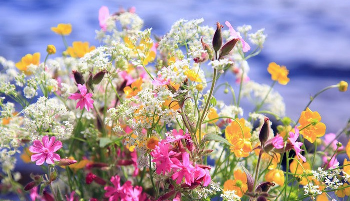
\includegraphics[width=.4\textheight]{fig/flowers}
                
                \begin{tabular}{c|c}
                    \hline\hline
                    Характеристика              & Оценка\\ \hline\hline
                    Безвредно                   & 5 \\
                    Обидно                      & 1 \\
                    Скрытно                     & 2 \\
                    Носимо                      & 4 \\
                    Дешево                      & 3 \\
                    Просто                      & 2 \\ 
                    Редко                       & 1 \\ \hline
                    \multicolumn{1}{r|}{Итого:} & $2.57\approx 3$ \\
                \end{tabular}
            \end{center}
    \end{columns}    
\end{frame}

Т.е. все оценки сложить и разделить на 7.

\subsection{Оценка существующих моделей}

\begin{frame}  %айфоня
    \begin{columns}
        \column{.50\textwidth}
            \begin{center}
                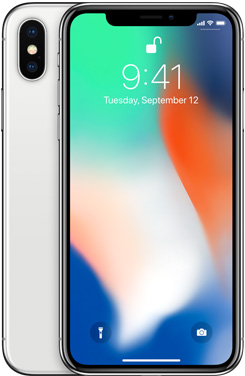
\includegraphics[height=.8\textheight]{fig/iphoneX}
            \end{center}
            
        \column{.40\textwidth}
            \begin{center}
                \begin{tabular}{c|c}
                    \hline\hline
                    Характеристика              & Оценка\\ \hline\hline
                    Безвредно                   & 1 \\
                    Обидно                      & 1 \\
                    Скрытно                     & 1 \\
                    Носимо                      & 5 \\
                    Дешево                      & 0 \\
                    Просто                      & 2 \\ 
                    Редко                       & 1 \\ \hline
                    \multicolumn{1}{r|}{Итого:} & $1.57\approx 2$ \\
                \end{tabular}
            \end{center}
    \end{columns}    
    
    Отвлекает \alert{всё} внимание от \alert{реальной жизни} на себя! Это \alert{не оружие} (см. оценки), а \alert{соперник}!
\end{frame}

Это оружие отвлекает все внимание на себя, а не привлекает внимание к хозяину. Проблема: iphoneX интереснее своего хозяина. Поэтому он вообще не является привниматическим оружием. Это оружие массового поражения, которое отвлекает внимание от реальной жизни на себя.

\begin{frame}  %духовая трубочка
    \begin{columns}
        \column{.50\textwidth}
            \begin{center}
                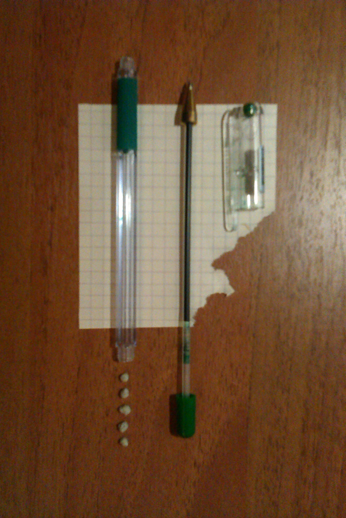
\includegraphics[width=.8\textwidth]{fig/airpipe}
            \end{center}
            
        \column{.40\textwidth}
            \begin{center}
                \begin{tabular}{c|c}
                    \hline\hline
                    Характеристика              & Оценка\\ \hline\hline
                    Безвредно                   & 4 \\
                    Обидно                      & 5 \\
                    Скрытно                     & 5 \\
                    Носимо                      & 5 \\
                    Дешево                      & 5 \\
                    Просто                      & 4 \\ 
                    Редко                       & 0 \\ \hline
                    \multicolumn{1}{r|}{Итого:} & $4$ \\
                \end{tabular}
            \end{center}
    \end{columns}    
\end{frame}

Духовая трубочка может быть сделана из любой ручки. Меткая стрельба требует тренировок.


\begin{frame} % рогатка из резиночки
    \begin{columns}
        \column{.50\textwidth}
            \begin{center}
                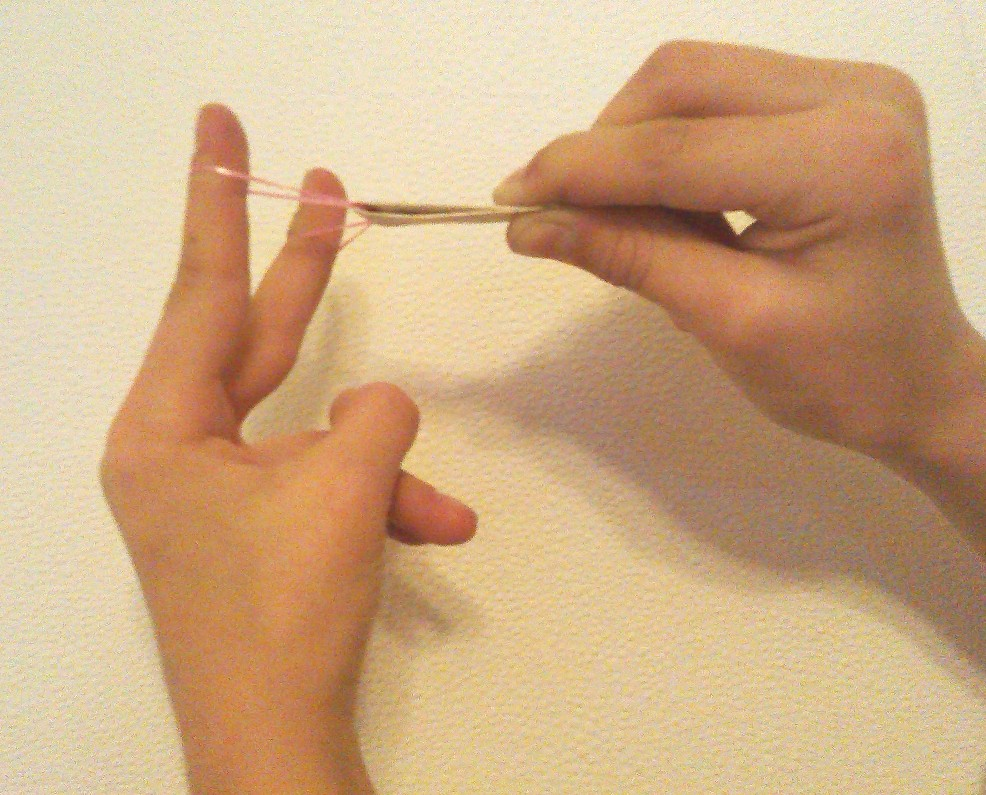
\includegraphics[width=\textwidth]{fig/slingshot}
            \end{center}
            
        \column{.40\textwidth}
            \begin{center}
                \begin{tabular}{c|c}
                    \hline\hline
                    Характеристика              & Оценка\\ \hline\hline
                    Безвредно                   & 4 \\
                    Обидно                      & 5 \\
                    Скрытно                     & 3 \\
                    Носимо                      & 3 \\
                    Дешево                      & 5 \\
                    Просто                      & 4 \\ 
                    Редко                       & 0 \\ \hline
                    \multicolumn{1}{r|}{Итого:} & $3.43\approx 3$ \\
                \end{tabular}
            \end{center}
    \end{columns}    
\end{frame}


\begin{frame} % резиночки сами по себе
    \begin{columns}
        \column{.50\textwidth}
            \begin{center}
                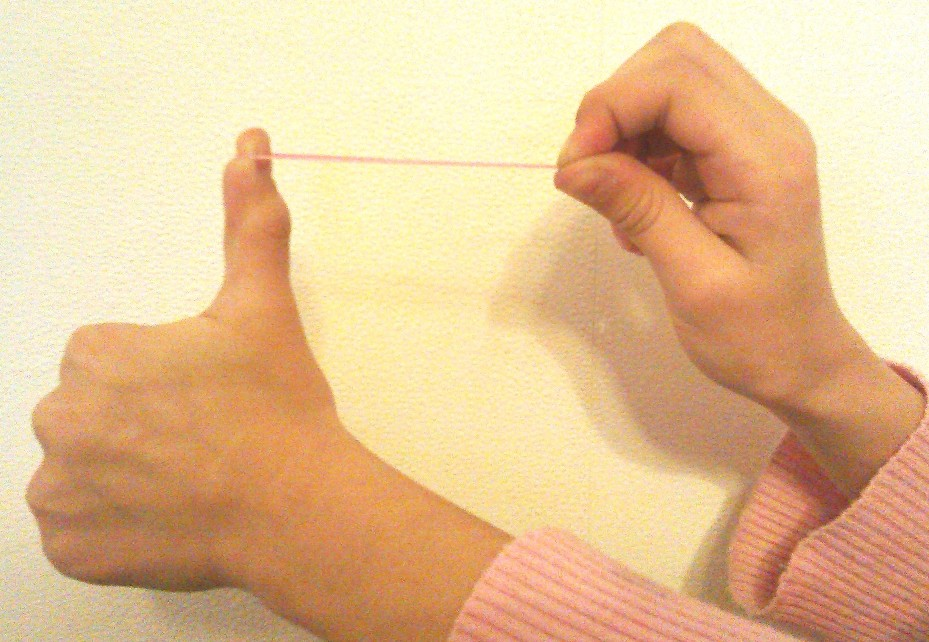
\includegraphics[width=\textwidth]{fig/elastic}
            \end{center}
            
        \column{.40\textwidth}
            \begin{center}
                \begin{tabular}{c|c}
                    \hline\hline
                    Характеристика              & Оценка\\ \hline\hline
                    Безвредно                   & 4 \\
                    Обидно                      & 5 \\
                    Скрытно                     & 5 \\
                    Носимо                      & 5 \\
                    Дешево                      & 4 \\
                    Просто                      & 4 \\ 
                    Редко                       & 0 \\ \hline
                    \multicolumn{1}{r|}{Итого:} & $3.86\approx 4$ \\
                \end{tabular}
            \end{center}
    \end{columns}    
\end{frame}

Экономический бум в Китае сделал резиночки для плетения очень доступными.

\begin{frame}
    \begin{center}
        Характеристики существующих образцов можно улучшить. 
        
        \par\bigskip
        
        Выполним разработку нового образча привниматического оружия.
    \end{center}
\end{frame}


\section{Создание и использование}

\begin{frame}
    \frametitle{\myDevice}
    %фото бзденьк
\end{frame}

\begin{frame}
    \frametitle{Режимы работы \myDevice}
    \framesubtitle{Переключаются отдельной кнопкой}
    
    \begin{itemize}
        \item вялый;
        \item импульсный;
        \item шквал.
    \end{itemize}    
\end{frame}

\subsection{Характеристики}

\begin{frame}
    \frametitle{\myDevice}
    \framesubtitle{Характеристики}
    
    \begin{columns}
        \column{.50\textwidth}
            %фото бзденька
        \column{.40\textwidth}
            \begin{center}
                \begin{tabular}{c|c}
                    \hline\hline
                    Характеристика              & Оценка\\ \hline\hline
                    Безвредно                   & 4 \\
                    Обидно                      & 5 \\
                    Скрытно                     & 4 \\
                    Носимо                      & 4 \\
                    Дешево                      & 3 \\
                    Просто                      & 5 \\ 
                    Редко                       & 4 \\ \hline
                    \multicolumn{1}{r|}{Итого:} & $3.86\approx 4$ \\
                \end{tabular}
            \end{center}
    \end{columns}    
\end{frame}


\subsection{Устройство}

\begin{frame}
    \frametitle{Механика \myDevice}
    
    %TODO: механика
\end{frame}

\begin{frame}
    \frametitle{Электроника \myDevice}
    
    \begin{center}
        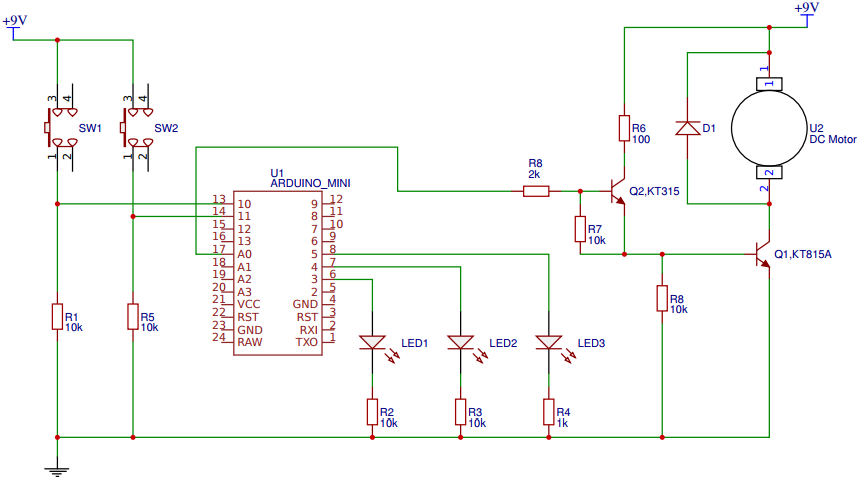
\includegraphics[width=0.99\textwidth]{fig/eScheme}
    \end{center}
\end{frame}

\begin{frame}
    \frametitle{Программирование контроллера \myDevice}
    
    \begin{center}
        
\includegraphics[width=0.4\textwidth]{fig/programming}
    \end{center}
\end{frame}

\begin{frame}
    \frametitle{Смета проекта \myDevice}
    
    \begin{center}
        \begin{tabular}{l|c|c|l}
            \hline\hline
            Деталь & Кол-во,шт. & Цена,руб. & Примечание \\
            \hline\hline
            Контроллер & 1  & 70   & Arduino Pro Mini,5V,16MHz\\
            Светодиод  & 3  & 0.50 & Красный, синий, зелёный\\
            Breadboard & 1  & 50   & Чтобы не паять детали\\
            Моторчик   & 1  & 50   & 4-9V, max 1A, 800 RPM\\
            Шестерёнки & 2  & 5    & Крутить обойму\\
            Батарейка  & 1  & 40   & Крона, 9V, питание схемы\\
            Провод     & -  & 0    & Нашли в папином ящике\\
            Транзистор & 2  & 0    & Нашли в папином ящике\\
            Изолента   & -  & 0    & Нашли в папином ящике\\
            Фанера     & -  & 0    & Нашли в гараже\\
            Деревяшка  & -  & 0    & Нашли в гараже\\
            Зубочистки & 17 & 0    & Нашли на кухне\\ \hline
            \multicolumn{2}{r|}{Итого(\alert{без учета работ}):} & \multicolumn{1}{c}{\alert{$221.50$}} & \\
        \end{tabular}
    \end{center}
\end{frame}


\subsection{Испытания \myDevice}

\begin{frame}
    \frametitle{Испытания \myDevice}
    \begin{center}
        В ходе испытаний ни одно живое существо не пострадало.

        Физически\ldots    
    \end{center}    
\end{frame}

\begin{frame}
    \frametitle{Испытание на котах}
    
    \begin{center}
        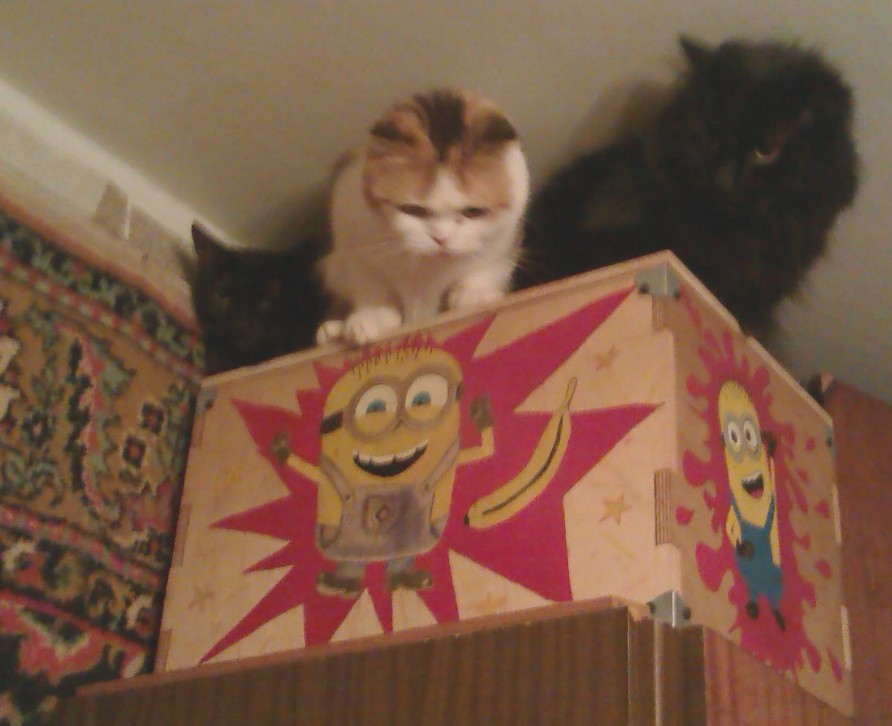
\includegraphics[width=0.7\textwidth]{fig/cats}
    \end{center}
\end{frame}

\begin{frame}
    \frametitle{Испытание на собаке}
    
    \begin{center}
        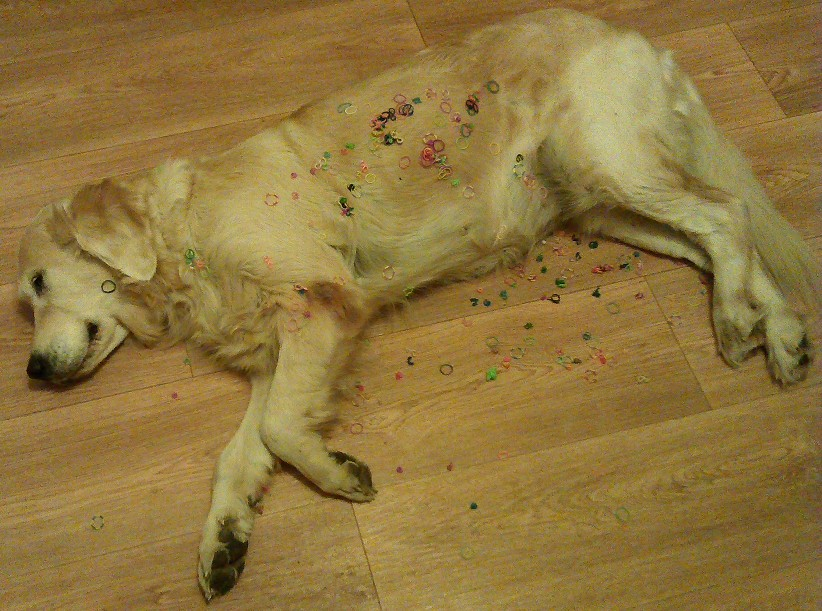
\includegraphics[width=0.75\textwidth]{fig/dog}
    \end{center}
\end{frame}

\begin{frame}
    \frametitle{Испытание на сестре}
    
    \begin{center}
        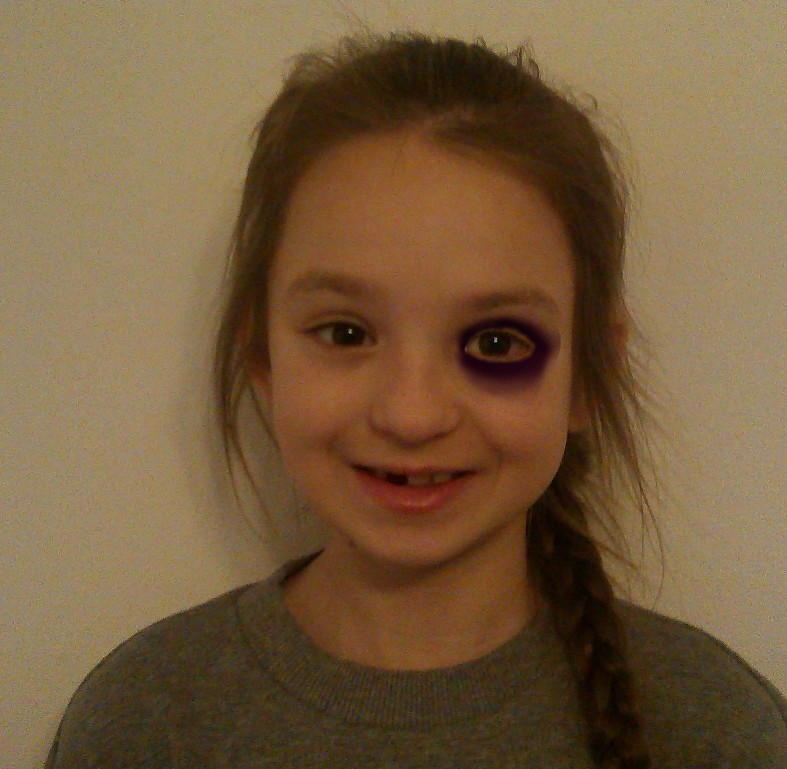
\includegraphics[width=0.6\textwidth]{fig/nastyaWork}
    \end{center}
\end{frame}

\begin{frame}
    \frametitle{Испытания на родителях}
    
    \begin{center}
        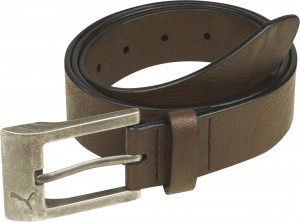
\includegraphics[width=.6\textwidth]{fig/belt}
    \end{center}
    
    Испытания на родителях решено не проводить\ldots
\end{frame}


\section{Оценки и выводы}


\subsection{Вывод по использованияю оружия}

\begin{frame}
    \frametitle{Вывод}
    
    Главный вывод звучит странно\ldots 
    
    \begin{block}{Главный вывод}
        Привнематическое оружие \alert{не должно} быть направлено на того, чье внимание нужно привлечь. 
    \end{block}
    
    \par\bigskip
    
    Лучше использовать его вместе, в дружеской игре --- тогда внимание будет \alert{взаимным} и \alert{добрым}.
\end{frame}


\subsection{Самое мощное\ldots}

\begin{frame}
    \frametitle{Заключение}
    
    Обобщив полученный опыт, можно с уверенностью утверждать, что:
    
    \begin{block}{}
        Самое мощное и \alert{единственное настоящее} привниматическое оружие --- это умный, сильный, увлекающийся, любопытный, а главное --- \alert{внимательный к окружающему миру} человек.
    \end{block}
\end{frame}

    
\subsection{Перспективы}

\begin{frame}
    \frametitle{Перспективы и направления развития}
    
    \begin{block}{Перспективы}
        \begin{center}
            Внимание \alert{каждому}!!!
        \end{center}
    \end{block}
    
    Направления развития \alert{настоящего} привнематического оружия: 
    \begin{itemize}
        \item искусство (музыка, танец, рисование, лепка, рукоделие,\ldots);
        \item наука (физика, математика, химия, биология, психология,\ldots);
        \item спорт (гимнастика, атлетика, плавание, боевые искусства,\ldots);
        \item помощь (людям, животным, растениям, чистоте улиц,\ldots);
        \item и т.д.
    \end{itemize}
    
    \begin{block}{}
        \begin{center}
            В \alert{одном} человеке могут сочетаться \alert{многие} направления, что повышает его \alert{мощность}, \alert{дальнобойность} и \alert{точность}.
        \end{center}
    \end{block}
    
\end{frame}


\appendix

\begin{frame}
    \frametitle{Литература, которая использовалась авторской группой}
    \framesubtitle{Пригодится для создания оружия из самого себя}

    Уверены, пригодится всем:
    \begin{itemize}
        \item создание характера в \cite{bib:kovey:sevenHabits};
        \item грамотный Русский язык привлекателен в \cite{bib:gal:WordLiveAndDeath}.
    \end{itemize}
    
    \par\bigskip
    
    Совсем не нужно тем, кому не очень интересно что такое:
    \begin{itemize}
        \item программирование \cite{bib:kernigan:practice};
        \item микроконтроллеры и электроника \cite{bib:margolis:Arduino}.
    \end{itemize}
\end{frame}

\begin{frame}[allowframebreaks]{Библиография}
    \bibliographystyle{unsrt}
    \bibliography{./../../../bibliobase}
\end{frame}

\begin{frame}
    \begin{center}
        \resizebox{\textwidth}{!}{Благодарю за \alert{внимание}!}
    \end{center}
    
    \par\bigskip
    
    \begin{center}
        Вопросы?
    \end{center}
    
\end{frame}

\end{document}